\subsection{Introducción}

\begin{frame}[plain]
  \centering
  \color{theme-brand-color}
  \Huge \textbf{Introducción}
\end{frame}

\begin{frame}{Motivación}
  Supongamos que queremos determinar si un valor \textit{x=9} pertenece a un arreglo $A$ de $N$ elementos.\\
  \begin{figure}[H]
    \centering
    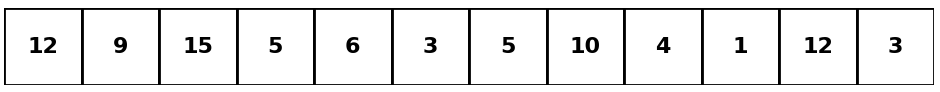
\includegraphics[width=0.85\textwidth]{./assets/array.png}
  \end{figure}
\end{frame}

\begin{frame}{Solución Naïve}
  Buscar uno por uno nos lleva tiempo lineal, para $Q$ queries sería $\bigO{QN}$.\\

  ¿Cómo lo podemos mejorar?
\end{frame}

\begin{frame}{Preprocesamiento}
  ¿Qué ocurre si $A$ esta ordenado? \\
  
  Podemos tomar un punto de referencia $i$ y plantear los siguientes casos:
  \begin{itemize}
  \item Si $a_i \leq x$, entonces $a_j \leq x$ para todo $j<i$.
  \item Si $x \leq a_i$, entonces $x \leq a_j$ para todo $i<j$.
  \item Si $x=a_i$, encontramos a $x$.
  \end{itemize}
\end{frame}

\begin{frame}{Idea}
  Considerar a un rango activo $[l,r]$ donde presumimos que estaría la respuesta (de estarlo), y a partir de un punto de referencia $i$ reducir el rango tan rápido como sea posible en el peor caso.\\

  En el peor caso reducimos el intervalo de $[l,r]$ a $max(i-l, r-i)$, por lo que el valor óptimo de $i=\lfloor\frac{l+r}{2} \rfloor$.
\end{frame}

\begin{frame}{Idea}
  \begin{figure}[H]
    \centering
    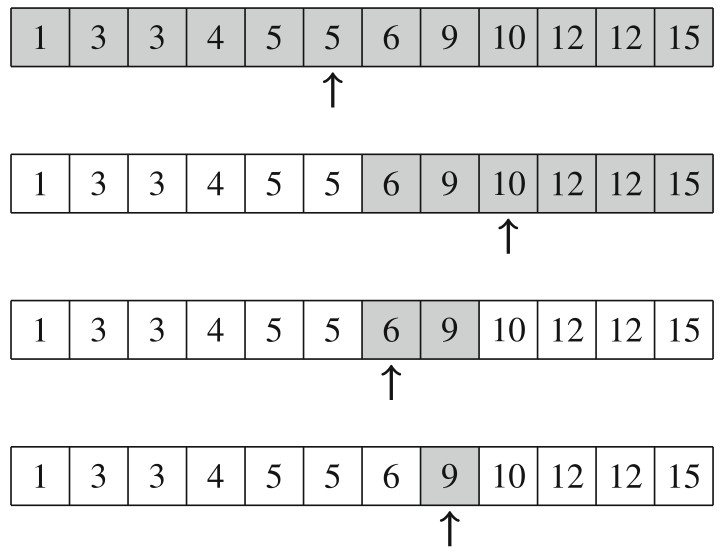
\includegraphics[width=0.65\textwidth]{./assets/idea.png}
  \end{figure}
\end{frame}

\begin{frame}[fragile]{Implementación}
\inputminted[
    fontsize=\large,
    linenos
]{cpp}{code/binary_search.cpp}
\end{frame}

\begin{frame}{Implementación}
  \begin{AlertP}
    Si $l+r$ excede el rango de \texttt{int}, este calculo se puede desbordar
    $$m = \frac{l+r}{2}$$

    La forma segura de hacerlo sería calcular
    $$m = l + \frac{r-l}{2}$$
  \end{AlertP}
\end{frame}

\begin{frame}{Complejidad}
  En cada iteración del algoritmo reducimos el rango activo a la mitad: \\

  $$N \rightarrow \frac{N}{2} \rightarrow \frac{N}{4} \rightarrow \cdots \rightarrow 1$$ \\

  Obteniendo una complejidad de $\bigO{\log N}$.
  
\end{frame}
